\chapter{Examples of usage of Grover's algorithm} \label{Practical_ch}

\section{Note on creating an oracle}
To understand how to create a quantum circuit that performs Grover's search, it is important to understand how to create an oracle. It is because the diffuser's matrix always has the same form, see sec. \ref{TeoreticalDiffuser}. Let us describe the pattern on the 3 following circuits.

\subsection{Basic concept}\label{basic_oracle}
We will show the most simple oracle on a circuit made with 2 qubits.
\begin{align}
\Qcircuit @C=1em @R=.7em {
& & & \psi_0 & &  & \psi_1 \\
 &\lstick{\ket{0}} &\qw& \gate{H}& \qw &\ctrl{1} &  \qw &\qw &\\
 &\lstick{\ket{0}} & \gate{X} & \gate{H}&\qw & \gate{X} &  \qw &\qw & \\
}
\end{align}

There, we are going to focus only on the first qubit, as it is the one that we are performing an oracle on.

At $\psi_0$ the first qubit is in state $|+\rangle$ and the second is in state $\psi_1$ is in state $|-\rangle$.
\begin{equation}
|\psi_0\rangle = |+\rangle \otimes |-\rangle = \frac{|0\rangle + |1\rangle}{\sqrt{2}} \otimes \frac{|0\rangle - |1\rangle}{\sqrt{2}} = \frac{(|0\rangle + |1\rangle)(|0\rangle - |1\rangle) }{2}.
\end{equation}
It is important to remember that the tensor product is not comutative.
\begin{equation}
|\psi_0\rangle = \frac{|00\rangle - |01\rangle + |10\rangle - |11\rangle }{2}.
\end{equation}
CNOT swaps the value at the second qubit if the first is $|1\rangle$. After CNOT operation we get $\psi_1$, which has the following form.

\begin{equation}
|\psi_1\rangle = \frac{|00\rangle - |01\rangle + |11\rangle - |10\rangle }{2}=\frac{|00\rangle - |01\rangle -(-|11\rangle) - |10\rangle }{2} = \frac{|0\rangle - |1\rangle}{\sqrt{2}} \otimes \frac{|0\rangle - |1\rangle}{\sqrt{2}}
\end{equation}
We see that the oracle has changed the value of $|1\rangle$, in the Grover's algorithm this means that $|1\rangle$ is the solution.
\subsection{Basic concept with X gate} \label{basic_oracle_x}
This time, we have almost the same circuit as before. The only difference is with a introduction of 2 X gates.

\begin{align}
\Qcircuit @C=1em @R=.7em {
& & & \psi_0 & \psi_1 &  \psi_2 & \psi_3 &  \\
 &\lstick{\ket{0}} & \gate{H} & \qw  &\gate{X} &\ctrl{1} &  \gate{X} &\qw &\\
 &\lstick{\ket{0}} & \gate{X} & \gate{H}& \qw & \gate{X} &  \qw &\qw & \\
}
\end{align}
First part will be same as in example one \ref{basic_oracle}.
\begin{equation}
|\psi_0\rangle = \frac{|00\rangle - |01\rangle + |10\rangle - |11\rangle }{2}.
\end{equation}
Switching the value of the first qubit with the X gate.
\begin{equation}
|\psi_1\rangle = \frac{|10\rangle - |11\rangle + |00\rangle - |01\rangle }{2}.
\end{equation}
Performing CNOT.
\begin{equation}
|\psi_2\rangle = \frac{|11\rangle - |10\rangle + |00\rangle - |01\rangle }{2}.
\end{equation}
Performing the X gate.
\begin{equation}
|\psi_3\rangle = \frac{-(-|01\rangle) - |00\rangle + |10\rangle - |11\rangle }{2} = \frac{-|0\rangle + |1\rangle}{\sqrt{2}} \otimes \frac{|0\rangle - |1\rangle}{\sqrt{2}}.
\end{equation}
This time we selected $|0\rangle$.
\subsection{Basic concept with multicontrol X gate}
This time, we will need 3 qubits.
\begin{align}
\Qcircuit @C=1em @R=.7em {
 && &\psi_0&\psi_1\\
 &\lstick{\ket{0}} &\qw&\gate{H}&\ctrl{2} &  \qw &\\
 &\lstick{\ket{0}} &\qw&\gate{H}&\ctrl{1} &  \qw &\\
 &\lstick{\ket{0}} & \gate{X}&\gate{H}&\gate{X} &  \qw &\\
}
\end{align}

\begin{equation}
|\psi_0\rangle = \frac{|0\rangle + |1\rangle}{\sqrt{2}} \otimes \frac{|0\rangle + |1\rangle}{\sqrt{2}} \otimes \frac{|0\rangle - |1\rangle}{\sqrt{2}}
\end{equation}

\begin{equation}
|\psi_0\rangle =  \frac{|000\rangle - |001\rangle +|010\rangle -|011\rangle +|100\rangle -|101\rangle + |111\rangle - |110\rangle}{2\sqrt{2}}
\end{equation}
After $CNOT_{0,1;2}$.

\begin{equation}
|\psi_1\rangle =  \frac{|00\rangle + |01\rangle + |10\rangle - |11\rangle }{2} \otimes \frac{|0\rangle - |1\rangle}{\sqrt{2}}.
\end{equation}

This time, the selected item was $|11\rangle$. To simply put it, multicontrol acting on $|-\rangle$ will set negative value only for the items (combinations) that perform the swapping on the controlled qubit, this is the reason why we had to switch the first qubit with the X gate in subsec. \ref{basic_oracle_x} to change the value of $|0\rangle$ to negative.

If we had more than one qubit, then selecting $|1\rangle$ on the first qubit would lead to selecting all combinations that have the feature. It would be, for example, $|1001\rangle$, $|1101\rangle$,...

\section{Circuit initialisation and diffuser}
There are multiple ways to create diffusers, we will focus on \cite{qc_grover_ibm}. We will show one that fits our definition and one that does not, but it works with different initialisation. Let us have $n+m+1$ qubits; then the diffuser on the first $n$ qubits that fits the definition will have the following form. It is good to clarify that the X and H gates are performed only on the first $n$ qubits and the second dots represent additional $m$ qubits. It is important to remember that there is a state $|-\rangle$ on the last qubit. 

\newpage
Uncompressed diffuser:
\begin{align}
\Qcircuit @C=1em @R=.7em {
 && &&&&&\\
&\qw & \gate{H} &\gate{X} &\ctrl{6} &\gate{X} &\gate{H} &\qw & \qw & \\
&\qw &\gate{H} &\gate{X} &\ctrl{5} &\gate{X} &\gate{H} & \qw & \qw & \\
&\qw &\gate{H} &\gate{X} &\ctrl{4} &\gate{X} &\gate{H} & \qw & \qw & \\
& &\vdots &\vdots &\vdots &\vdots &\vdots &\\
&& &&&&&\\
 &\qw &\gate{H} &\gate{X} &\ctrl{2} &\gate{X} &\gate{H} &\qw & \qw & \\
 & &\vdots &\vdots &\vdots &\vdots &\vdots &\\
 &\qw & \qw & \qw & \gate{X} &\qw & \qw &\qw &  \\
}
\end{align}
Compressed diffuser:
\begin{align}
\Qcircuit @C=1em @R=.7em {
 && &&&&&\\
&\qw & \gate{H} &\ctrl{6}  &\gate{H} &\qw & \qw & \\
&\qw &\gate{H} &\ctrl{5}  &\gate{H} & \qw & \qw & \\
&\qw &\gate{H}  &\ctrl{4}  &\gate{H} & \qw & \qw & \\
& &\vdots &\vdots &\vdots &\\
&& &&&&&\\
 &\qw &\gate{H}  &\ctrl{2} &\gate{H} &\qw & \qw & \\
 & &\vdots &\vdots &\vdots &\\
 &\qw & \qw  & \gate{X} &\qw  &\qw  &\qw \\
}
\end{align}
Initialisation part for compressed diffuser:

\begin{align}
\Qcircuit @C=1em @R=.7em {
 && &&&&&\\
 &\lstick{\ket{0}} &\gate{X}&\gate{H}\\
 &\lstick{\ket{0}} &\gate{X}&\gate{H}\\
 &\lstick{\ket{0}} &\gate{X}&\gate{H}\\
 & &\vdots &\vdots &\\
  && &&&&&\\
 &\lstick{\ket{0}} &\gate{X}&\gate{H}\\
 & &\vdots &\vdots &\\
 && &&&&&\\
 &\lstick{\ket{0}} & \gate{X}&\gate{H}&\\
}
\end{align}

\section{Small Sudoku}

We will start with a small example. The task is taken from \cite{qc_grover_ibm}. The problem is the following; find the combinations that fit into the following clauses. The first clause is $v_0 \neq v_1 $, the second is $v_0 \neq v_2 $, the third is $v_1 \neq v_3 $ and the last is $v_2 \neq v_3 $, where $v_0, v_1, v_2, v_3 \in \{ 0,1 \}$.

\begin{figure}[h!]
\begin{center}
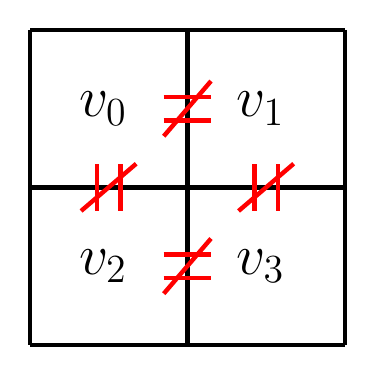
\begin{tikzpicture}


\draw[black, ultra thick] (0,0) -- (4,0);
\draw[black, ultra thick] (0,4) -- (0,0);
\draw[black, ultra thick] (4,4) -- (0,4);
\draw[black, ultra thick] (4,4) -- (4,0);


\draw[black, ultra thick] (0,2) -- (4,2);
\draw[black, ultra thick] (2,0) -- (2,4);

\draw[black] (0.5,3) node[anchor=west,font=\huge]{$v_0$};
\draw[black] (2.5,3) node[anchor=west,font=\huge]{$v_1$};
\draw[black] (0.5,1) node[anchor=west,font=\huge]{$v_2$};
\draw[black] (2.5,1) node[anchor=west,font=\huge]{$v_3$};

\draw[red, ultra thick] (1.7,0.85) -- (2.3,0.85);
\draw[red, ultra thick] (1.7,1.15) -- (2.3,1.15);
\draw[red, ultra thick] (1.7,0.65) -- (2.3,1.35);


\draw[red, ultra thick] (1.7,2.85) -- (2.3,2.85);
\draw[red, ultra thick] (1.7,3.15) -- (2.3,3.15);
\draw[red, ultra thick] (1.7,2.65) -- (2.3,3.35);

\draw[red, ultra thick] (2.85,1.7) -- (2.85,2.3);
\draw[red, ultra thick] (3.15,1.7) -- (3.15,2.3);
\draw[red, ultra thick] (2.65,1.7) -- (3.35,2.3);

\draw[red, ultra thick] (0.85,1.7) -- (0.85,2.3);
\draw[red, ultra thick] (1.15,1.7) -- (1.15,2.3);
\draw[red, ultra thick] (0.65,1.7) -- (1.35,2.3);


\end{tikzpicture}
\caption{Task visualisation} \label{small_sudoku_vis}
\end{center}
\end{figure}






From the observation of the assign, we are able to construct the following equations. Note that the following functions are going to be boolean.
\begin{equation} \label{1st_condition}
    (v_0 \cdot \overline{v_1})+(\overline{v_0} \cdot v_1) = 1
\end{equation}

\begin{equation} \label{2nd_condition}
    (v_0 \cdot \overline{v_2})+(\overline{v_0} \cdot v_2) = 1
\end{equation}

\begin{equation} \label{3rd_condition}
    (v_2 \cdot \overline{v_3})+(\overline{v_3} \cdot v_2) = 1
\end{equation}
We won't cover simple solution in \cite{qc_grover_ibm}, instead, we will focus on smaller solutions, that can run on currently available quantum computers. 

\subsection{Solution with 6 qubits} \label{Solution_with_6_qubits}

The first solution requires 6 qubits, which is a large improvement over the original 9 presented by IBM; the trick is to compact the oracle from 9 to 6 qubits. We will use the following picture to show states during the run of the algorithm. This solution was proposed by the supervisor, Jiří Tomčala, Ph.D.

\begin{align}
\Qcircuit @C=1em @R=.7em {
 &\psi_0& &&&  &&&&&&\psi_1\\
&\qw &\ctrl{4} &  \qw & \ctrl{2} &\qw&\qw&\qw&\ctrl{2}&\qw&\ctrl{4}\qw&\qw&\\
&\qw&\qw & \ctrl{3}\qw &  \qw&\ctrl{2} &\qw&\ctrl{2} &\qw&\ctrl{3}&\qw&\qw&\\
  &\qw&  \qw &  \qw &\gate{X}& \qw &\ctrl{3}&\qw&\gate{X}  &\qw&\qw&\qw&\\
 &\qw&    \qw &  \qw &\qw &\gate{X}&\ctrl{2} &\gate{X}&\qw&\qw&\qw&\qw&\\
 &\qw&\gate{X} &\gate{X} &  \qw &\qw &\ctrl{1} &\qw  &\qw &\gate{X}&\gate{X}&\qw&\\
 &\qw &  \qw &\qw &\qw &\qw &\gate{X} &\qw  &\qw &\qw &\qw&\qw&\\
}
\end{align}
The trick there is we use qubits both for storing value of our result as well as for implementing clauses. The first two CNOTs implement simple functions so that the first and second qubits cannot have the same value. As we pointed out before, the qubit has to be $|1\rangle$ to transfer the negative phase. The third CNOT can be interpreted as the first qubit being not equal to the third. The same goes for the second qubit, where CNOT implements XOR between the second and the fourth qubit. CNOTs after CCCNOT implement some sort of cleaning, so that oracle performs only phase rotation and nothing more. 

To derive states during the run of the algorithm, we will use an uncompressed diffuser, we will observe only states on the first four qubits, as the vector of all 6 qubits would have length of 64.

\begin{align}
\Qcircuit @C=1em @R=.7em {
&\psi_1&\psi_2&\psi_3&\psi_4&\psi_5&\psi_6&&\\
&\qw & \gate{H} &\gate{X} &\ctrl{5} &\gate{X} &\gate{H} &\qw & \qw & \\
&\qw &\gate{H} &\gate{X} &\ctrl{4} &\gate{X} &\gate{H} & \qw & \qw & \\
&\qw &\gate{H} &\gate{X} &\ctrl{3} &\gate{X} &\gate{H} & \qw & \qw & \\
&\qw &\gate{H} &\gate{X} &\ctrl{2} &\gate{X} &\gate{H} &\qw & \qw & \\
&\qw&\qw&\qw&\qw&\qw&\qw&\qw&\qw\\
 &\qw & \qw & \qw & \gate{X} &\qw & \qw &\qw &\qw \\
}
\end{align}
Let $\mathcal{T}=\{1001,0110\} $ and $\mathcal{F}=\{0,1\}^4 \setminus \mathcal{T}$

\begin{equation}
    |\psi_0\rangle =  \sum_{i\in \{0,1\}^4}^{} \frac{|i\rangle }{4}.
\end{equation}

\begin{equation}
    |\psi_1\rangle =  \sum_{i\in \mathcal{F}}^{} \frac{|i\rangle }{4} -\sum_{i\in \mathcal{T}}^{} \frac{|i\rangle }{4}.
\end{equation}

\begin{equation}
    |\psi_2\rangle =  \frac{3}{4}|0000\rangle+\frac{1}{4}|0011\rangle+\frac{1}{4}|0101\rangle-\frac{1}{4}|0110\rangle-\frac{1}{4}|1001\rangle+\frac{1}{4}|1010\rangle+\frac{1}{4}|1100\rangle-\frac{1}{4}|1111\rangle.
\end{equation}

\begin{equation}
    |\psi_3\rangle = \frac{1}{4}|0000\rangle-\frac{1}{4}|0011\rangle-\frac{1}{4}|0101\rangle+\frac{1}{4}|0110\rangle+\frac{1}{4}|1001\rangle-\frac{1}{4}|1010\rangle-\frac{1}{4}|1100\rangle-\frac{3}{4}|1111\rangle.
\end{equation}

\begin{equation}
    |\psi_4\rangle = \frac{1}{4}|0000\rangle-\frac{1}{4}|0011\rangle-\frac{1}{4}|0101\rangle+\frac{1}{4}|0110\rangle+\frac{1}{4}|1001\rangle-\frac{1}{4}|1010\rangle-\frac{1}{4}|1100\rangle+\frac{3}{4}|1111\rangle.
\end{equation}

\begin{equation}
    |\psi_5\rangle = \frac{3}{4}|0000\rangle-\frac{1}{4}|0011\rangle-\frac{1}{4}|0101\rangle+\frac{1}{4}|0110\rangle+\frac{1}{4}|1001\rangle-\frac{1}{4}|1010\rangle-\frac{1}{4}|1100\rangle+\frac{1}{4}|1111\rangle.
\end{equation}

\begin{equation}
    |\psi_6\rangle =  \sum_{i\in \mathcal{F}}^{} \frac{|i\rangle }{8} -\sum_{i\in \mathcal{T}}^{} \frac{5|i\rangle }{8}.
\end{equation}

We can check the results with our recurrence eqs. \ref{multi_solution_lambda_last} and \ref{multi_solution_theta_last}. Let $\Theta_0 = \frac{1}{4}$, $\Lambda_0 = \frac{1}{4}$, $m = 2$, and $n = 4$.

\begin{equation}
    \Lambda_1 = (1-\frac{2\cdot2}{16})\frac{1}{4} + (16-2)\frac{2}{16}\frac{1}{4}=\frac{12}{64}+\frac{28}{64} = \frac{40}{64} = \frac{5}{8}.
\end{equation}

\begin{equation}
    \Theta_1 = -\frac{2}{16}\cdot2\cdot\frac{1}{4} + (1-\frac{2\cdot 2}{16})\frac{1}{4} = \frac{-4}{64}+\frac{12}{64} = \frac{8}{64} = \frac{1}{8}.
\end{equation}
This is exactly the result of simulating our algorithm. We ran algorithm on IBM's device Ibm\_nairobi with following results.

\begin{figure}[H]
\centering
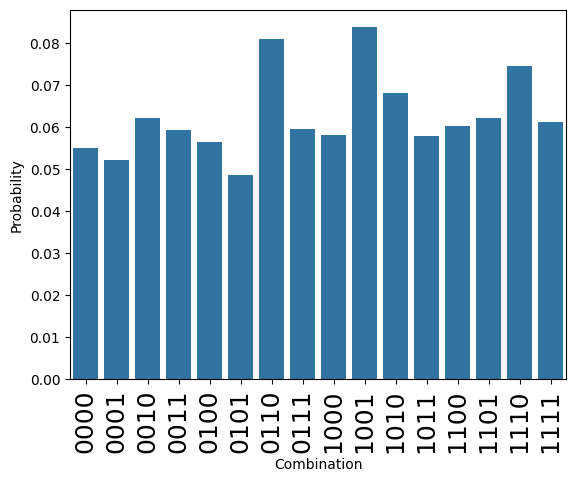
\includegraphics[width=10cm]{Figures/bc0_0.png}
\caption{Results from the QC}
\label{Smallb00}
\end{figure}

Result from simulator:
\begin{figure}[H]
\centering
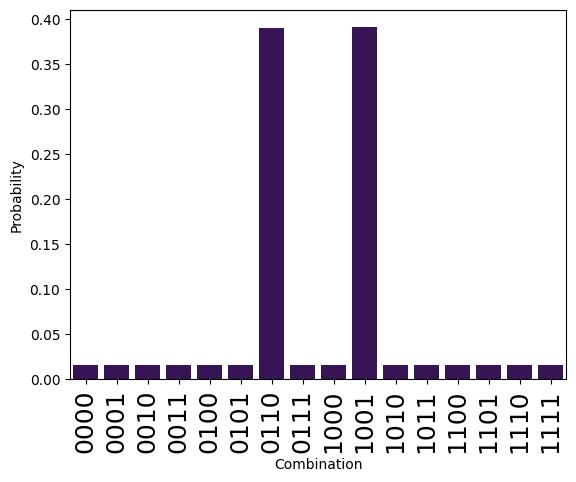
\includegraphics[width=10cm]{Figures/sim0.png}
\caption{Results from the simulator}
\label{sim0}
\end{figure}


We see that even with that small circuit there is a lot of noise, in fig. \ref{Smallb00} the most two observed results are the correct solution to the given problem, but it is easy to see that many other incorrect solutions are observed more, than theoretical computations predicted. The simulation results are comparable to the theoretical values.

\subsection{Solution with 5 qubits}

Now, we are going to focus on equations \ref{1st_condition}, \ref{2nd_condition} and \ref{3rd_condition}, which must be true at the same time, leading to the following expression.
\begin{equation}
    \Bigl( \big(v_0 \cdot \overline{v_1})+(\overline{v_0} \cdot v_1) \Bigl) \cdot \Bigl( (v_0 \cdot \overline{v_2})+(\overline{v_0} \cdot v_2) \Bigl) \cdot \Bigl( (v_2 \cdot \overline{v_3})+(\overline{v_2} \cdot v_3) \Bigl) = 1.
\end{equation}
After distribution,

\begin{equation}
    \Bigl( \big(v_0 \cdot \overline{v_1})+(\overline{v_0} \cdot v_1) \Bigl) \cdot \Bigl( (v_0 \cdot \overline{v_2})+(\overline{v_0} \cdot v_2) \Bigl) \cdot  (v_2 \cdot \overline{v_3})+\Bigl( \big(v_0 \cdot \overline{v_1})+(\overline{v_0} \cdot v_1) \Bigl) \cdot \Bigl( (v_0 \cdot \overline{v_2})+(\overline{v_0} \cdot v_2) \Bigl)(\overline{v_2} \cdot v_3)  = 1.
\end{equation}
Further after second distribution,

\begin{equation}
    \begin{multlined}
        \Bigl( \big(v_0 \cdot \overline{v_1})+(\overline{v_0} \cdot v_1) \Bigl) \cdot \Bigl( (v_0 \cdot \overline{v_2})+(\overline{v_0} \cdot v_2) \Bigl) \cdot  (v_2 \cdot \overline{v_3})+ 
        \\
        \Bigl( \big(v_0 \cdot \overline{v_1})+(\overline{v_0} \cdot v_1) \Bigl) \cdot ( (v_0 \cdot \overline{v_2}) \cdot (\overline{v_2} \cdot v_3) + 
        \\
        \Bigl( \big(v_0 \cdot \overline{v_1})+(\overline{v_0} \cdot v_1) \Bigl) \cdot (\overline{v_0} \cdot v_2) \cdot (\overline{v_2} \cdot v_3) = 1.
        \end{multlined}
\end{equation}  
Sice $A\overline{A}=0$,

\begin{equation}
    \begin{multlined}
        \Bigl( \big(v_0 \cdot \overline{v_1})+(\overline{v_0} \cdot v_1) \Bigl) \cdot \Bigl( (v_0 \cdot \overline{v_2})+(\overline{v_0} \cdot v_2) \Bigl) \cdot  (v_2 \cdot \overline{v_3})+ 
        \\
        \Bigl( \big(v_0 \cdot \overline{v_1})+(\overline{v_0} \cdot v_1) \Bigl) \cdot ( (v_0 \cdot \overline{v_2}) \cdot (\overline{v_2} \cdot v_3) = 1.
        \end{multlined}
\end{equation}
$AA=A$,
\begin{equation}
    \begin{multlined}
        \Bigl( \big(v_0 \cdot \overline{v_1})+(\overline{v_0} \cdot v_1) \Bigl) \cdot \Bigl( (v_0 \cdot \overline{v_2})+(\overline{v_0} \cdot v_2) \Bigl) \cdot  (v_2 \cdot \overline{v_3})+ 
        \\
        \Bigl( \big(v_0 \cdot \overline{v_1})+(\overline{v_0} \cdot v_1) \Bigl) \cdot  (v_0 \cdot \overline{v_2} \cdot v_3) = 1.
        \end{multlined}
\end{equation}
After another distribution.

\begin{equation}
    \begin{multlined}
        \Bigl( \big(v_0 \cdot \overline{v_1})+(\overline{v_0} \cdot v_1) \Bigl) \cdot \Bigl( (v_0 \cdot \overline{v_2})+(\overline{v_0} \cdot v_2) \Bigl) \cdot  (v_2 \cdot \overline{v_3})+ 
        \\
        ( v_0 \cdot \overline{v_1})(v_0 \cdot \overline{v_2} \cdot v_3) + (\overline{v_0} \cdot v_1)(v_0 \cdot \overline{v_2} \cdot v_3) = 1.
        \end{multlined}
\end{equation}
$A\overline{A}=0$ and $AA=A$
\begin{equation}
    \begin{multlined}
        \Bigl( \big(v_0 \cdot \overline{v_1})+(\overline{v_0} \cdot v_1) \Bigl) \cdot \Bigl( (v_0 \cdot \overline{v_2})+(\overline{v_0} \cdot v_2) \Bigl) \cdot  (v_2 \cdot \overline{v_3})+ v_0 \cdot \overline{v_1} \cdot \overline{v_2} \cdot v_3 =1
        \end{multlined}
\end{equation}
Let us apply same steps onto the first part of the equation aswell. 

\begin{equation}
    \begin{multlined}
        \Bigl( \big(v_0 \cdot \overline{v_1})+(\overline{v_0} \cdot v_1) \Bigl) \cdot \Bigl((v_0 \cdot \overline{v_2})(v_2 \cdot \overline{v_3})+(\overline{v_0} \cdot v_2)(v_2 \cdot \overline{v_3})\Bigl) +
        \\
        v_0 \cdot \overline{v_1} \cdot \overline{v_2} \cdot v_3 =1
        \end{multlined}
\end{equation}
Apply identities,
\begin{equation}
    \begin{multlined}
        \Bigl( \big(v_0 \cdot \overline{v_1})+(\overline{v_0} \cdot v_1) \Bigl) \cdot \Bigl( (\overline{v_0} \cdot v_2 \cdot \overline{v_3}\Bigl) +
        v_0 \cdot \overline{v_1} \cdot \overline{v_2} \cdot v_3 =1.
        \end{multlined}
\end{equation}
Applying last distribution,

\begin{equation}
    \begin{multlined}    
        v_0 \cdot \overline{v_1} \cdot\overline{v_0} \cdot v_2 \cdot \overline{v_3} + \overline{v_0} \cdot v_1 \cdot \overline{v_0} \cdot v_2 \cdot  \overline{v_3}+
        v_0 \cdot \overline{v_1} \cdot \overline{v_2} \cdot v_3 =1.
        \end{multlined}
\end{equation}
$A\overline{A}=0$ gives
\begin{equation}
    \begin{multlined}    
       \overline{v_0} \cdot v_1 \cdot v_2 \cdot \overline{v_3}+
        v_0 \cdot \overline{v_1} \cdot \overline{v_2} \cdot v_3 =1.
        \end{multlined}
\end{equation}

This means that we have 2 representations of the same function, we can give a quantum computer to compute. We can also see that the term at the end is shorter and uses fewer gates. The down side of this solution is in CCCCNOT gates, in the original solution there was only one, there are three of them. Such a gate is decomposed into multiple CNOTs and other gates. This leads to the conclusion that this may be more compact, but it will run longer on a quantum computer, thus, more incorrect measurements will be observed.
Oracle:
\begin{align}
\Qcircuit @C=1em @R=.7em {
&\psi_0 & & &\psi_1&&&\psi_2&&\\
&\qw  &\gate{X} &\ctrl{4} &\gate{X}&\qw &\ctrl{4} &\qw  &\qw & \qw & \\
&\qw  & \qw &\ctrl{3} &\qw&\gate{X} &\ctrl{3} &\gate{X}  & \qw & \qw & \\
&\qw  &\qw &\ctrl{2} &\qw&\gate{X} &\ctrl{2} &\gate{X}  & \qw & \qw & \\
&\qw  &\gate{X} &\ctrl{1} &\gate{X}&\qw &\ctrl{1} &\qw  &\qw & \qw & \\
 &\qw & \qw & \gate{X} &\qw & \qw & \gate{X} & \qw & \qw & \qw \\
}
\end{align}
Diffuser:
\begin{align}
\Qcircuit @C=1em @R=.7em {
&\psi_2&\psi_3&\psi_4&\psi_5&\psi_6&\psi_7&&\\
&\qw & \gate{H} &\gate{X} &\ctrl{4} &\gate{X} &\gate{H} &\qw & \qw & \\
&\qw &\gate{H} &\gate{X} &\ctrl{3} &\gate{X} &\gate{H} & \qw & \qw & \\
&\qw &\gate{H} &\gate{X} &\ctrl{2} &\gate{X} &\gate{H} & \qw & \qw & \\
&\qw &\gate{H} &\gate{X} &\ctrl{1} &\gate{X} &\gate{H} &\qw & \qw & \\
 &\qw & \qw & \qw & \gate{X} &\qw & \qw &\qw &\qw \\
}
\end{align}

\begin{equation}
    |\psi_0\rangle =  \sum_{i\in \{0,1\}^4}^{} \frac{|i\rangle }{4}.
\end{equation}

\begin{equation} \label{psi1_small}
    |\psi_1\rangle =  \sum_{i\in \{0,1\}^4\setminus 0110}^{} \frac{|i\rangle }{4} -\frac{|0110\rangle }{4}.
\end{equation}

\begin{equation}
    |\psi_2\rangle =  \sum_{i\in \mathcal{F}}^{} \frac{|i\rangle }{4} -\sum_{i\in \mathcal{T}}^{} \frac{|i\rangle }{4}.
\end{equation}

\begin{equation}
    |\psi_3\rangle =  \frac{3}{4}|0000\rangle+\frac{1}{4}|0011\rangle+\frac{1}{4}|0101\rangle-\frac{1}{4}|0110\rangle-\frac{1}{4}|1001\rangle+\frac{1}{4}|1010\rangle+\frac{1}{4}|1100\rangle-\frac{1}{4}|1111\rangle.
\end{equation}

\begin{equation}
    |\psi_4\rangle = \frac{1}{4}|0000\rangle-\frac{1}{4}|0011\rangle-\frac{1}{4}|0101\rangle+\frac{1}{4}|0110\rangle+\frac{1}{4}|1001\rangle-\frac{1}{4}|1010\rangle-\frac{1}{4}|1100\rangle-\frac{3}{4}|1111\rangle.
\end{equation}

\begin{equation}
    |\psi_5\rangle = \frac{1}{4}|0000\rangle-\frac{1}{4}|0011\rangle-\frac{1}{4}|0101\rangle+\frac{1}{4}|0110\rangle+\frac{1}{4}|1001\rangle-\frac{1}{4}|1010\rangle-\frac{1}{4}|1100\rangle+\frac{3}{4}|1111\rangle.
\end{equation}

\begin{equation}
    |\psi_6\rangle = \frac{3}{4}|0000\rangle-\frac{1}{4}|0011\rangle-\frac{1}{4}|0101\rangle+\frac{1}{4}|0110\rangle+\frac{1}{4}|1001\rangle-\frac{1}{4}|1010\rangle-\frac{1}{4}|1100\rangle+\frac{1}{4}|1111\rangle.
\end{equation}

\begin{equation}
    |\psi_7\rangle =  \sum_{i\in \mathcal{F}}^{} \frac{|i\rangle }{8} -\sum_{i\in \mathcal{T}}^{} \frac{5|i\rangle }{8}.
\end{equation}

After eq. \ref{psi1_small} the algorithm has the same states as \ref{Solution_with_6_qubits}, but it is not surprising as we only made a different oracle and described it in two steps instead of one.

This time we used IBM's Ibm\_nairobi and got the following results.

\begin{figure}[h]
\centering
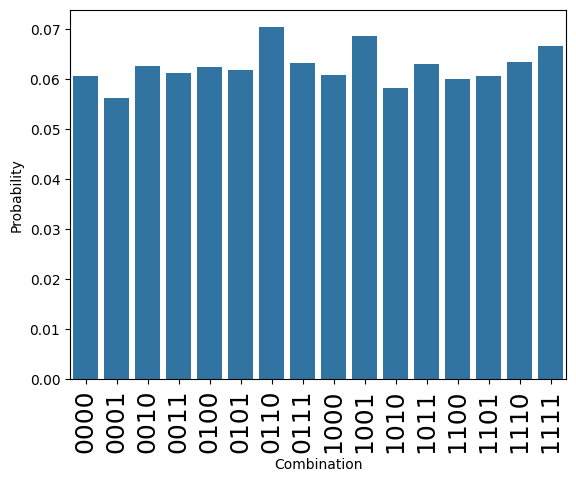
\includegraphics[width=10cm]{Figures/bc1_0.png}
\caption{Results from the QC}
\label{Smallb10}
\end{figure}
Result from simulator:
\begin{figure}[H]
\centering
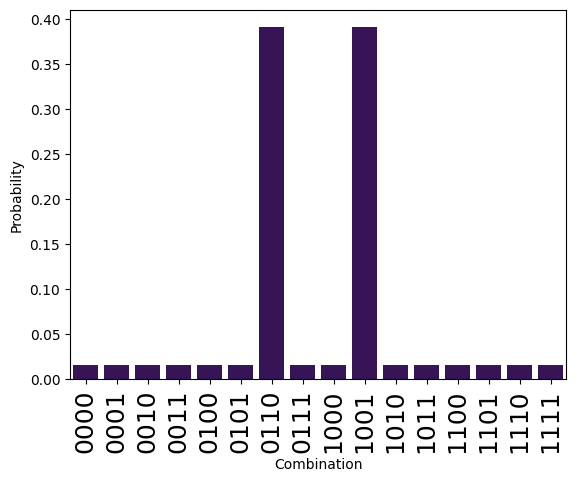
\includegraphics[width=10cm]{Figures/sim1.png}
\caption{Results from the simulator}
\label{sim1}
\end{figure}

We see a similar trend as before, where we have a good result in fig. \ref{Smallb10}, but it is incomparable with \ref{sim1}, where we see that the counts are close to theoretical values. Compared to fig. \ref{Smallb00} we have worse results, as incorrect combinations are measured more, but still the two most measured combinations are solution to the given problem.
\section{Large Sudoku}

We are given a 3x3 grid, in each tile, there can be either 0 or 1. In each row and in each column the sum must be 2.

\begin{figure}[h!]
\begin{center}
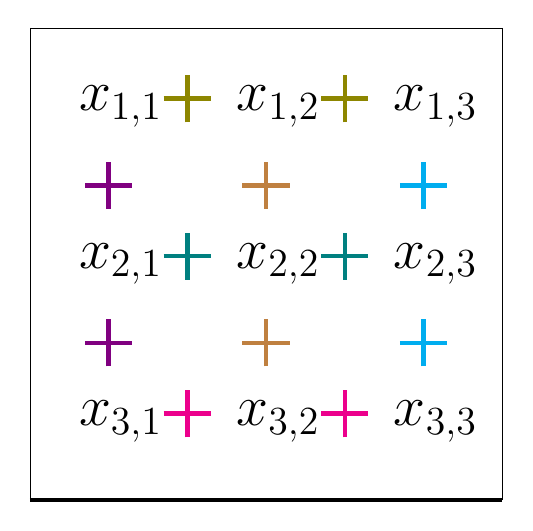
\begin{tikzpicture}


\draw[black, ultra thick] (0,0) -- (6,0);
\draw[black, ultra thin] (0,6) -- (0,0);
\draw[black,ultra  thin] (6,6) -- (0,6);
\draw[black,ultra  thin] (6,6) -- (6,0);

%\draw[black,ultra  thin] (0,2) -- (6,2);
%\draw[black,ultra  thin] (0,4) -- (6,4);

%\draw[black,ultra  thin] (2,0) -- (2,6);
%\draw[black,ultra  thin] (4,0) -- (4,6);

\draw[black] (0.5,1) node[anchor=west,font=\huge]{$x_{3,1}$};
\draw[black] (2.5,1) node[anchor=west,font=\huge]{$x_{3,2}$};
\draw[black] (4.5,1) node[anchor=west,font=\huge]{$x_{3,3}$};

\draw[black] (0.5,3) node[anchor=west,font=\huge]{$x_{2,1}$};
\draw[black] (2.5,3) node[anchor=west,font=\huge]{$x_{2,2}$};
\draw[black] (4.5,3) node[anchor=west,font=\huge]{$x_{2,3}$};

\draw[black] (0.5,5) node[anchor=west,font=\huge]{$x_{1,1}$};
\draw[black] (2.5,5) node[anchor=west,font=\huge]{$x_{1,2}$};
\draw[black] (4.5,5) node[anchor=west,font=\huge]{$x_{1,3}$};

\draw[violet, ultra thick] (0.7,2) -- (1.3,2);
\draw[violet, ultra thick] (1,1.7) -- (1,2.3);

\draw[violet, ultra thick] (0.7,4) -- (1.3,4);
\draw[violet, ultra thick] (1,3.7) -- (1,4.3);

\draw[brown, ultra thick] (2.7,2) -- (3.3,2);
\draw[brown, ultra thick] (3,1.7) -- (3,2.3);

\draw[brown, ultra thick] (2.7,4) -- (3.3,4);
\draw[brown, ultra thick] (3,3.7) -- (3,4.3);

\draw[cyan, ultra thick] (4.7,2) -- (5.3,2);
\draw[cyan, ultra thick] (5,1.7) -- (5,2.3);

\draw[cyan, ultra thick] (4.7,4) -- (5.3,4);
\draw[cyan, ultra thick] (5,3.7) -- (5,4.3);

\draw[magenta, ultra thick] (2,0.8) -- (2,1.4);
\draw[magenta, ultra thick] (1.7,1.1) -- (2.3,1.1);

\draw[magenta, ultra thick] (4,0.8) -- (4,1.4);
\draw[magenta, ultra thick] (3.7,1.1) -- (4.3,1.1);

\draw[teal, ultra thick] (2,2.8) -- (2,3.4);
\draw[teal, ultra thick] (1.7,3.1) -- (2.3,3.1);

\draw[teal, ultra thick] (4,2.8) -- (4,3.4);
\draw[teal, ultra thick] (3.7,3.1) -- (4.3,3.1);

\draw[olive, ultra thick] (2,4.8) -- (2,5.4);
\draw[olive, ultra thick] (1.7,5.1) -- (2.3,5.1);

\draw[olive, ultra thick] (4,4.8) -- (4,5.4);
\draw[olive, ultra thick] (3.7,5.1) -- (4.3,5.1);


\end{tikzpicture}
\caption{Task visualisation} \label{large_sudoku_vis}
\end{center}
\end{figure}

We see that there are six sums, which means that we have six different clauses, which will constitute our oracle. The number of correct combinations can be computed from understanding that there will always be only one 0 in the current row and column. For the first selection of
a row and a column, we have three options; after putting down 0 here, there are only two options for a second row and a column. After repeating the process, the last place has only one option. This means that $m=3\cdot2\cdot 1=6$.

To understand the concept of this oracle, we have to understand the following circuit. Here, we will choose the position of our 0 in a row or column. $Impacted$ qubit will be in state $|1\rangle$ if exactly one of the controlling qubits in combination is $|1\rangle$ or all three are in a state $|1\rangle$, to avoid
selecting $|111\rangle$ as valid, we have to put here a CCCNOT - then for $|111\rangle$ will be in a state $impacted =|0\rangle$ . 


\begin{align}
\Qcircuit @C=1em @R=.7em {
 && &&&&&\\
 &\lstick{q_a} &\ctrl{5}&\qw& \qw &\ctrl{5}&\qw\\
 &\lstick{q_b} &\qw&\ctrl{4}& \qw &\ctrl{4}&\qw\\
 &\lstick{q_c} &\qw&\qw& \ctrl{3}&\ctrl{3}&\qw\\
 & \vdots & & &   &\\
  && &&&&&\\
 &\lstick{impacted} &\gate{X}&\gate{X} & \gate{X}& \gate{X}&\qw\\
 & \vdots &\\
 && &&&&&\\
 &\lstick{\ket{-}} & \qw & \qw &\qw &\qw &\qw\\
}
\label{simp_oracle_large}
\end{align}

We will continue with circ. \ref{simp_oracle_large}. To implement all 6 conditions, we will use the following set: $\mathcal{S} = \Bigl\{(1,2,3,10),(4,5,6,11),(7,8,9,12),(1,4,7,13),(2,5,8,14),(3,6,9,15)\Bigl\}$, where numbers represent a qubit's index, indexing from 1. Then the oracle will have the following structure: we will encode all six foursomes so that $(q_a,q_b,q_c,impacted) \in \mathcal{S}$, then $CNOT_{10,11,12,13,14,15|16}$, with $q_{16}=|-\rangle$ and again $(q_a,q_b,q_c,impacted) \in \mathcal{S}$.

It is important to remember that we picked position for 0, in correct combination the position will be 1, on the other hand all other positions will be 0 but in our task, they should be labelled as 1. To fix this we add a layer of X gates on the first 9 qubits after the last application of the diffuser.

This time we have only access to the simulator for running the task. We got the following results.

With performing only one iteration we can see from the plot that correct combinations have probability to be measured circa $0.017$, incorrect $0.0019$.

\begin{figure}[H]
\centering
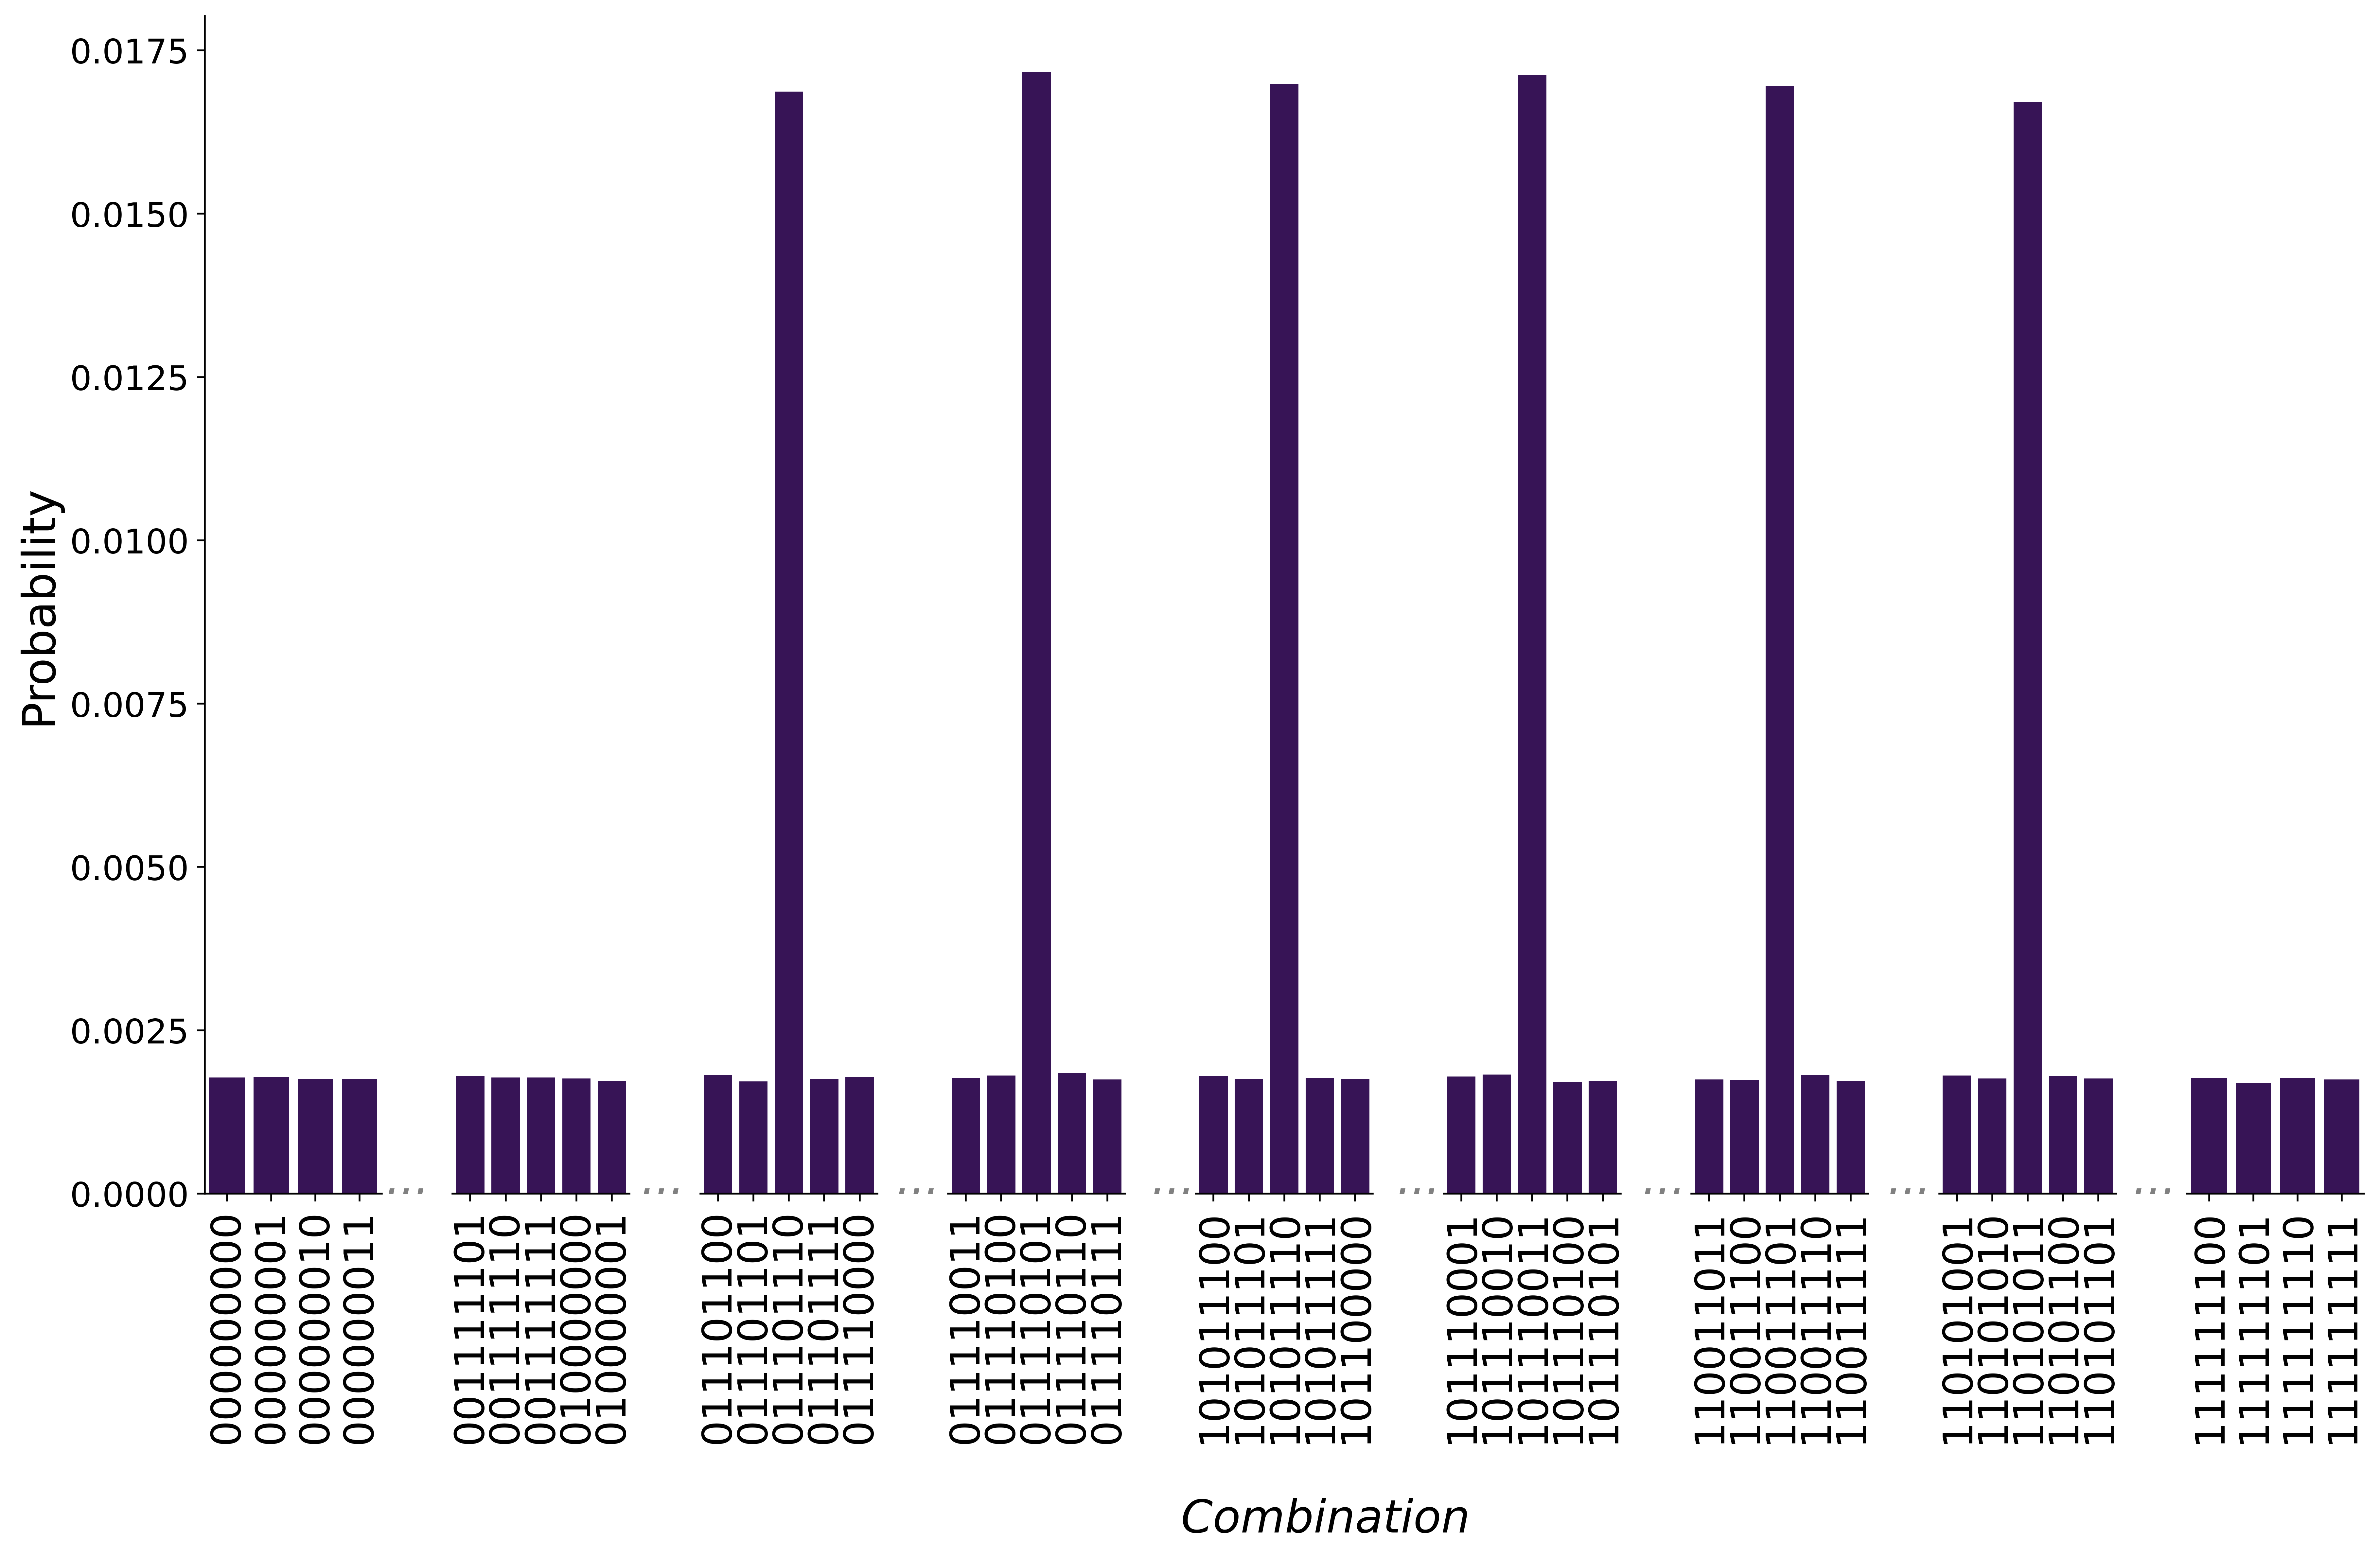
\includegraphics[width=18cm]{Figures/large1iter.png}
\caption{Results from the simulator with one iteration}
\label{After first iteration}
\end{figure}

With performing only one iteration we can see from the plot that correct combinations have probability to be measured circa $0.017$, incorrect less than $0.002$.

\begin{figure}[H]
\centering
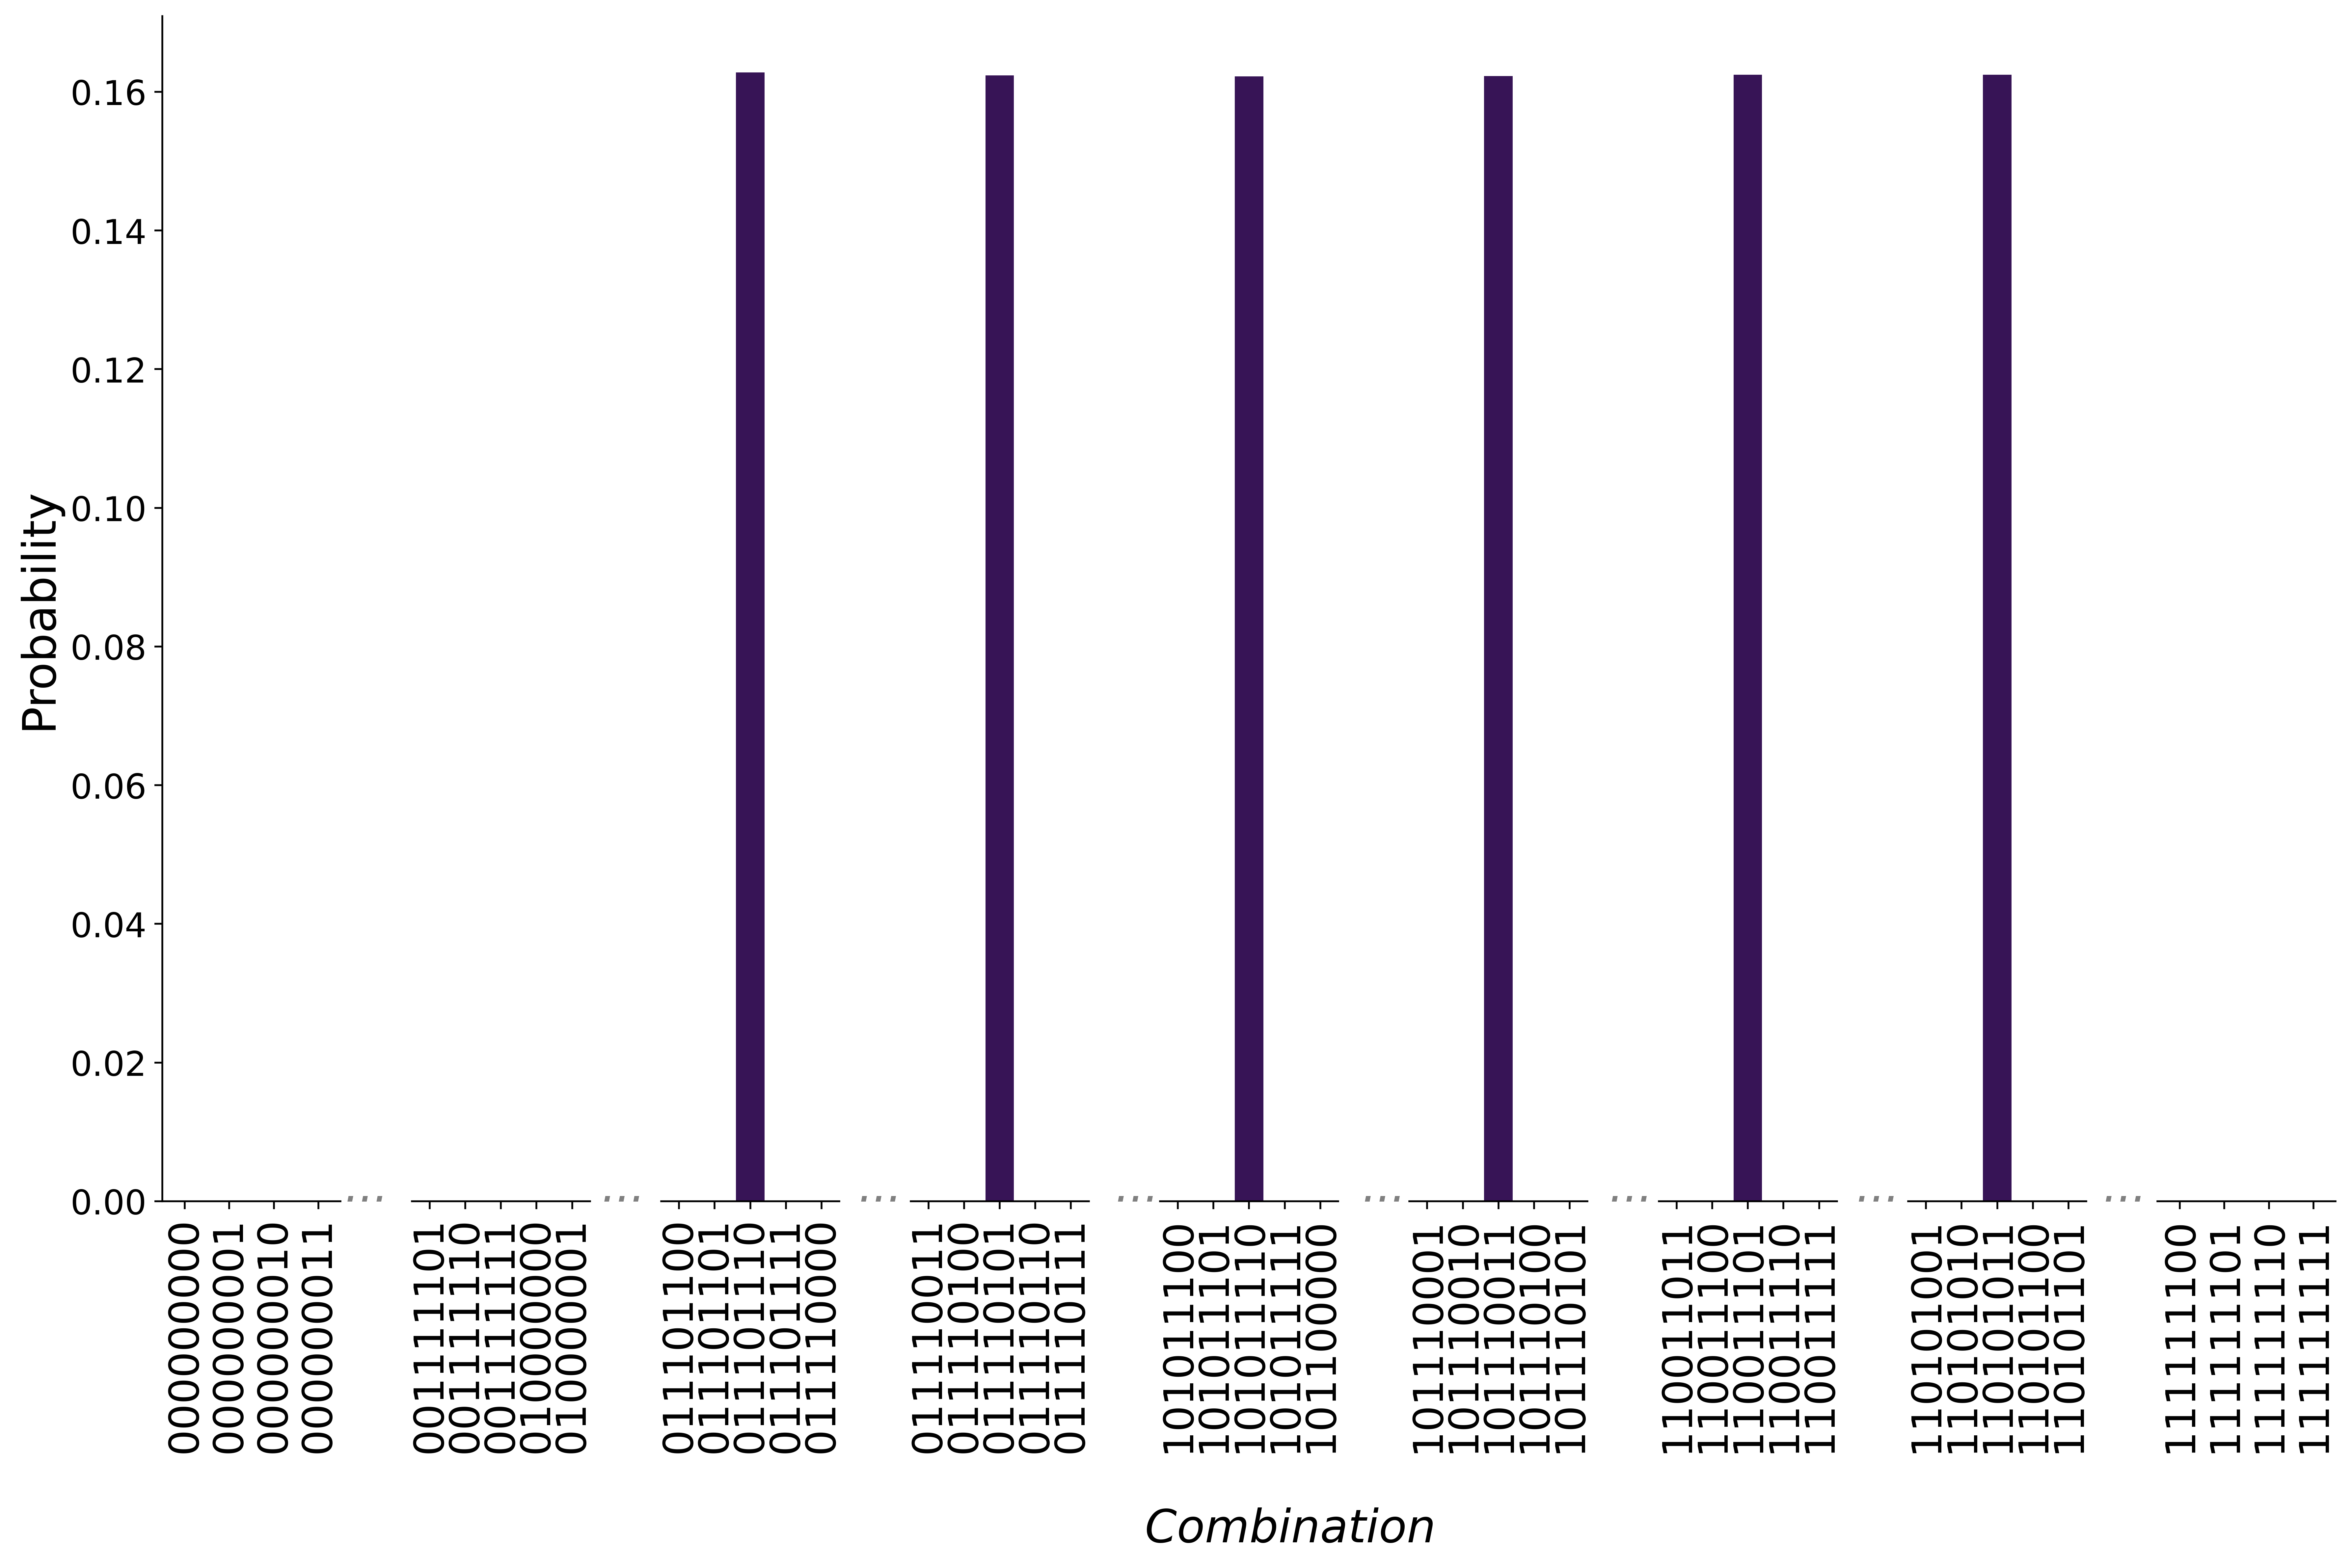
\includegraphics[width=17cm]{Figures/largefinal.png}
\caption{Results from the simulator}
\label{sim_large}
\end{figure}

When we perform optimal number of iterations (in this case, 6 or 7), we get almost ten times improvement with measuring the correct combinations. We also see that there is a very small probability of measuring one of the other $506$ combinations.

It is also important not to confuse that the solution is periodical. With the decimal representation, the results could be interpreted as $\{238, 245, 350, 371, 413, 427\}$. Despite not having any reasonable metric, we can see that intuitively they are distributed unequally.
